%Performance analysis
Simulation of an IEEE network is carried out in EMTP-RV for determining the short circuit capability of CB under different fault conditions. The results are obtained for the following fault conditions.
\begin{enumerate}
\item Interruption of three phase to ground fault at the terminal of substation for switching multiple lines connected to the substation

\item Interruption of three phase to ground fault at the terminal of substation for the case of transformer switching

\item Interruption of single phase to ground short line fault and modeling the line as constant parameter and frequency dependent and comparing the results for the two

\item Interruption of three phase to ground fault at the terminal of substation with arc model
\end{enumerate}

\section{Computational Analysis}

\subsection{Simulation results for case-I}
Simulation is carried out for interruption of three phase to ground fault at the terminal of the substation for switching multiple lines connected to the substation. Stray capacitance of substation equipments is considered for simulation. Current in the steady state under fault condition is measured which is 17.2 kA. For a breaker of 30 kA short circuit interruption capabilities, the standard TRV for T60 duty is modeled by four parameter method. The rating of TRV for T60 duty is obtained from the application guide shown in the Table \ref{table:: TRV Rating for 30 kA Short Circuit Current Interruption}.The simulation time step of 1$\mu s$ is used. The standard TRV and the TRV across the breaker is shown in the waveforms from figure \ref{Fig:4.1.1} to figure \ref{Fig:4.1.3}. The TRV waveform is exponential as seen in figure \ref{Fig:4.1.3}. In this case when the CB is used to switch the multiple lines, CB has inductance and capacitance on source side as well as on the load side which results in double frequency recovery voltage.

\subsection{Simulation results for case-II}
Simulation is carried out for interruption of three phase to ground fault at the terminal of a substation for the case of transformer switching. The simulation time step of 1$\mu s$ is used. As seen in the waveforms from figure \ref{Fig:4.1.4} to figure \ref{Fig:4.1.7}, the TRV is oscillatory since the fault is limited by the transformer only. The electric energy is redistributed among equivalent single capacitive and single inductive elements. In this case since the CB is used for transformer switching with no transmission lines, the circuit becomes underdamped and the resulting TRV is a typical one minus cosine waveform.

\subsection{Simulation results for case-III}
Simulation is carried out for interruption of single phase to ground short line fault at various fault distance from 1.2 km to 6.2 km for a 16 km transmission line. The lines are first modeled in constant parameter mode, and TRV is recorded. Then the lines are modeled in frequency dependent mode, and TRV is recorded. TRV in both models is compared. Time step of 0.1 $\mu s$ is used. Obtained waveforms are shown from figure \ref{Fig:4.1.8} to figure \ref{Fig:4.1.15}. The reflections of the travelling waves against short circuit point and the open end at the breaker side causes a triangular shaped waveform. The increase in line length increases the line impedance and the amplitude of the triangular shaped line side oscillation which decreases the fault current; hence $di/dt$ becomes lower. The characteristic impedance $Z_{line}$ depends on the line parameters and remains constant. Hence the RRRV decreases with increase in line length and vice-versa.

\subsection{Simulation results for arc interruption}
Simulation is carried out for interruption of three phase to ground fault at the terminal of a substation for switching multiple lines connected to the substation as well as transformer switching. Black Box Cassie-Mayer model is used for arc interruption studies. Time step of 0.1 $\mu s$ is used. The waveforms are shown in figure \ref{Fig:4.1.16} to figure \ref{Fig:4.1.17}.

\begin{sidewaystable}[!htbp]
\renewcommand{\arraystretch}{1.3}
\caption{TRV Rating for 30 kA Short Circuit Current Interruption}
\label{table:: TRV Rating for 30 kA Short Circuit Current Interruption}
\centering
\small
\begin{tabular}{ | >{\centering\arraybackslash}m{0.7in} | >{\centering\arraybackslash}m{0.7in} | >{\centering\arraybackslash}m{0.7in} | >{\centering\arraybackslash}m{0.7in} | >{\centering\arraybackslash}m{0.7in} | >{\centering\arraybackslash}m{0.5in} | >{\centering\arraybackslash}m{0.7in} | >{\centering\arraybackslash}m{0.5in} | >{\centering\arraybackslash}m{0.5in} | >{\centering\arraybackslash}m{0.6in} | >{\centering\arraybackslash}m{0.5in} | >{\centering\arraybackslash}m{0.7in} | } \hline
Rated voltage & Test duty & First pole to clear factor & Amplitude factor & First reference voltage & Time & TRV Peak value & Time & Time delay & Voltage & Time & Rate of rise \\ \hline
U1& & kpp & kaf & u1 & t1 	& uc & t2 or t3 & Td   & U' & t'   & u1/t1 \\
kV& & 	  & 	& kV &$\mu$s& uc & $\mu$s	&$\mu$s& kV &$\mu$s& uc/t3 \\
	& & & & & & & & & & 									& kV/$\mu$s \\ \hline

\multirow{5}{*}{145} &T100&1.3& 1.40& 115& 58& 215& 232& 2(16)& 58& 31(45)& 2 \\ \cline{2-12}
&\textbf{T60}& \textbf{1.3}& \textbf{1.50}& \textbf{115}& \textbf{38}& \textbf{231}& \textbf{228}& \textbf{2-12}& \textbf{58}& \textbf{21-31}& \textbf{3} \\ \cline{2-12}
&T30& 1.3& 1.54& -& -& 237& 47& 7& 79& 23& 5 \\ \cline{2-12}
&T10& 1.5& 0.9$\times$1.7& -& -& 272& 39& 6& 91& 19& 7 \\ \cline{2-12}
&Op1-Op2& 2& 1.25& 178& 178& 296& 232-464& 2-12& 89& 60-70& 1.54 \\ \hline
\end{tabular}
\end{sidewaystable}

\begin{sidewaysfigure}
   \centering 
   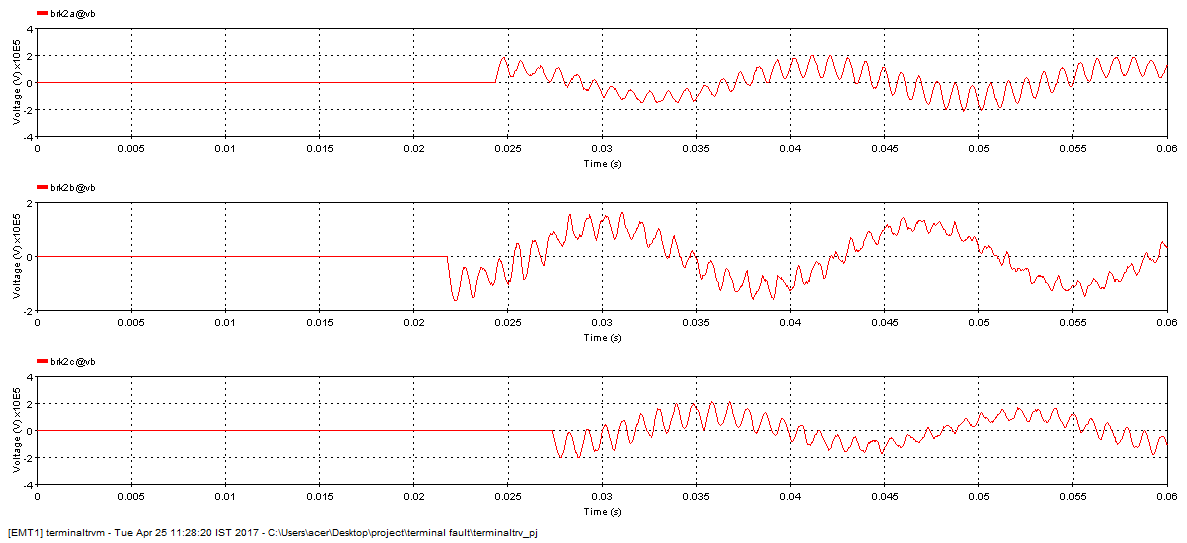
\includegraphics[width=\textwidth]{1trvcb2p2411} 
   \caption{TRV Waveform of the Three Phases for Multiple Line Switching at Terminal of Substation for Three Phase to Ground Fault}
   \label{Fig:4.1.1} 
\end{sidewaysfigure}

%***********************************************************************************************

\begin{sidewaysfigure}
   \centering 
   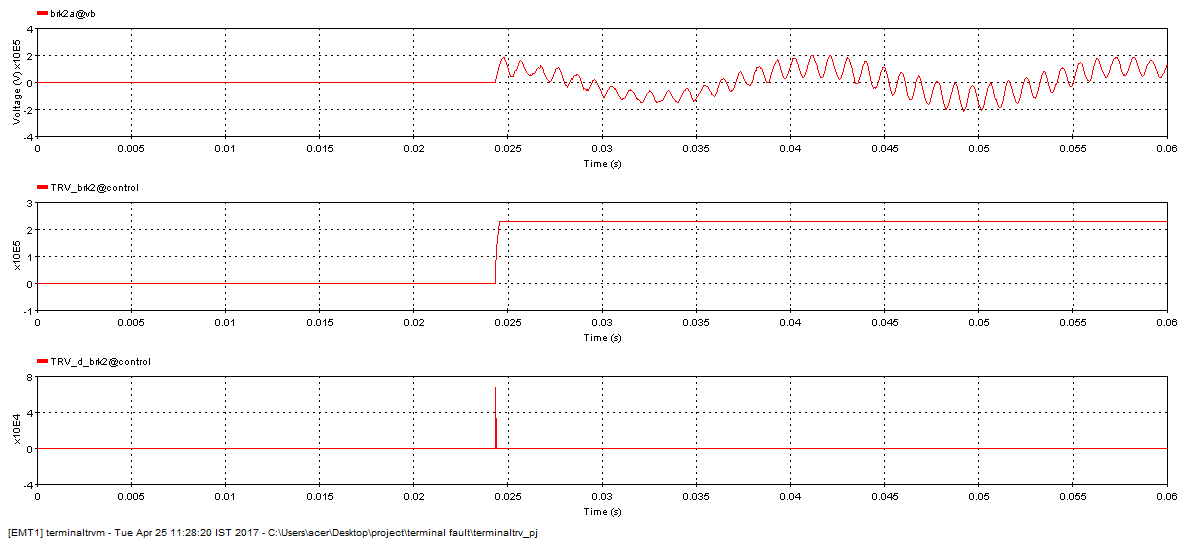
\includegraphics[width=\textwidth]{2trvawithstdcbp2412} 
   \caption{TRV Waveform of Phase A with Standard TRV and Delay Line for Multiple Line Switching at Terminal of Substation for Three Phase to Ground Fault}
   \label{Fig:4.1.2} 
\end{sidewaysfigure}

%***********************************************************************************************

\begin{sidewaysfigure}
   \centering 
   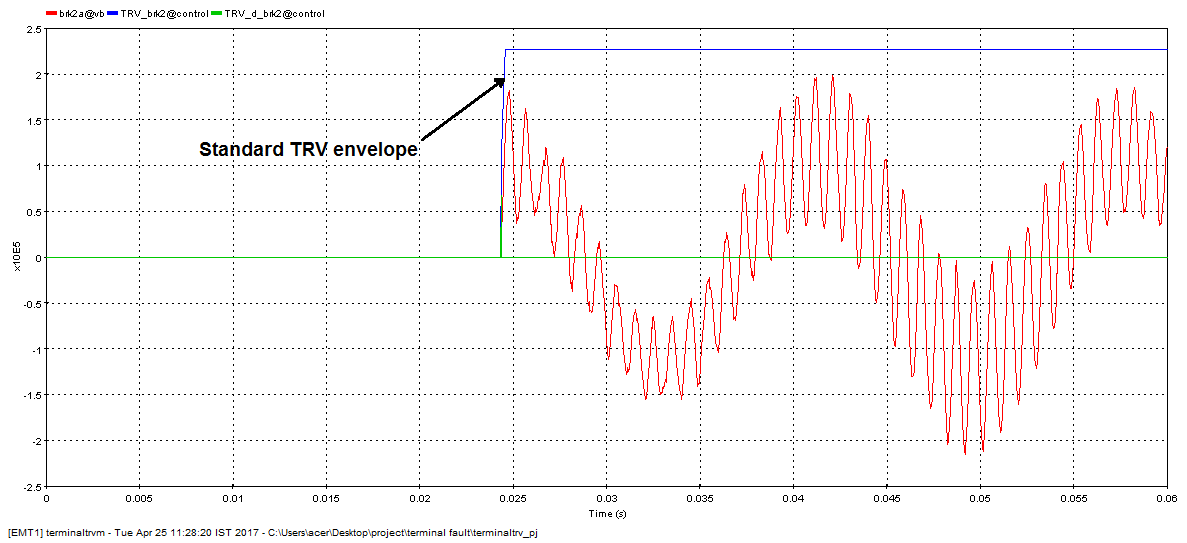
\includegraphics[width=\textwidth]{3trvawithstdenlargedcbp2413} 
   \caption{Standard TRV Envelope and Phase A TRV for Multiple Line Switching at Terminal of Substation for Three Phase to Ground Fault}
   \label{Fig:4.1.3} 
\end{sidewaysfigure}

%***********************************************************************************************

\begin{sidewaysfigure}
   \centering 
   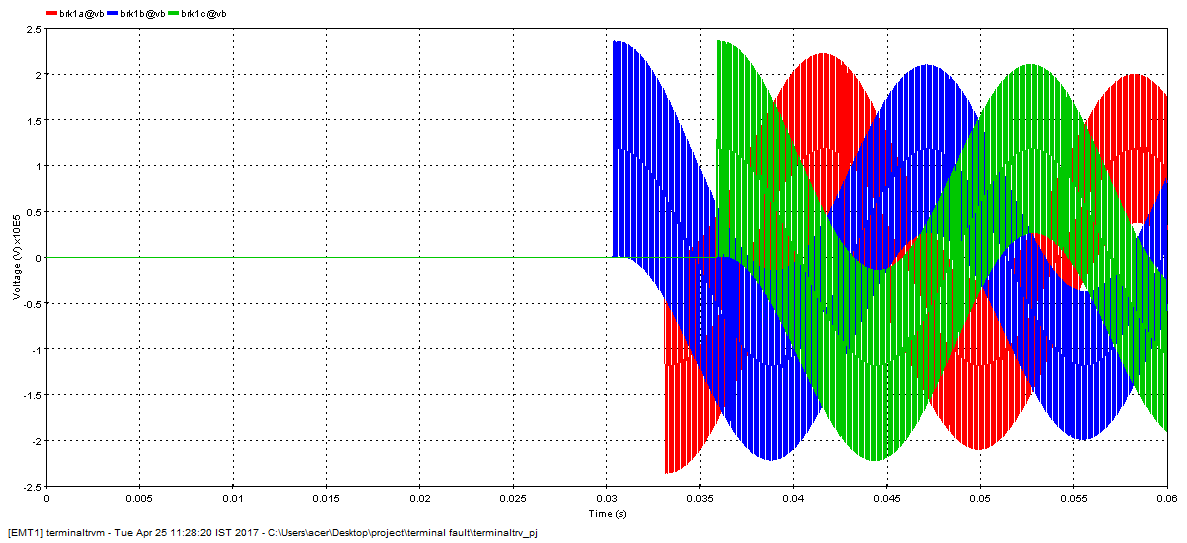
\includegraphics[width=\textwidth]{4completetrvcb1p1414} 
   \caption{Oscillatory TRV for Three Phase to Ground Terminal Fault for Transformer Switching}
   \label{Fig:4.1.4} 
\end{sidewaysfigure}

%***********************************************************************************************

\begin{sidewaysfigure}
   \centering 
   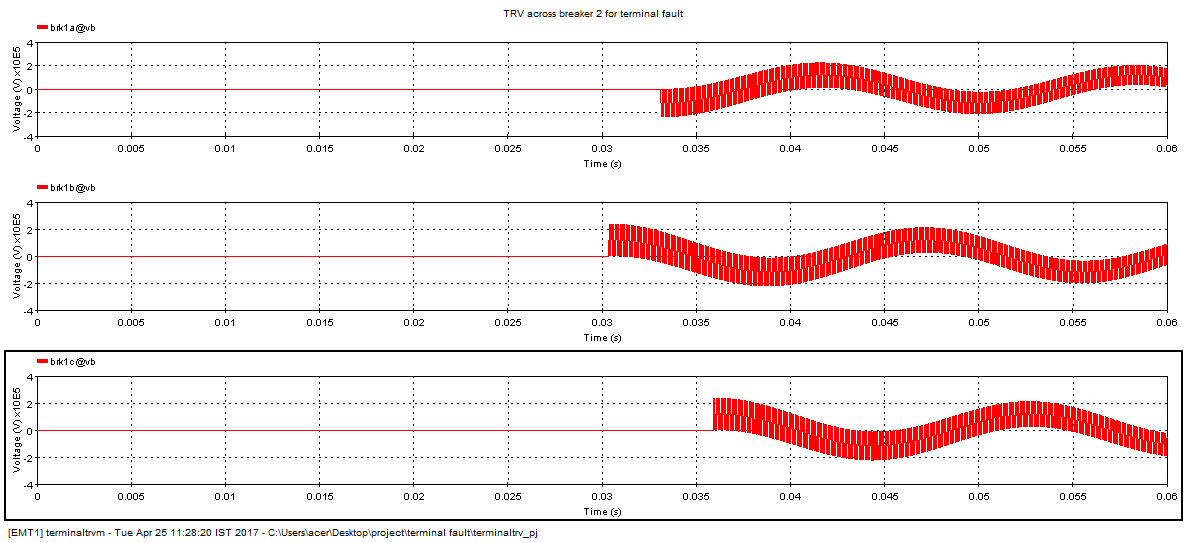
\includegraphics[width=\textwidth]{5trvcb1p1415} 
   \caption{Three Phase Oscillatory TRV for Three Phase to Ground Terminal Fault for Transformer Switching}
   \label{Fig:4.1.5} 
\end{sidewaysfigure}

%***********************************************************************************************

\begin{sidewaysfigure}
   \centering 
   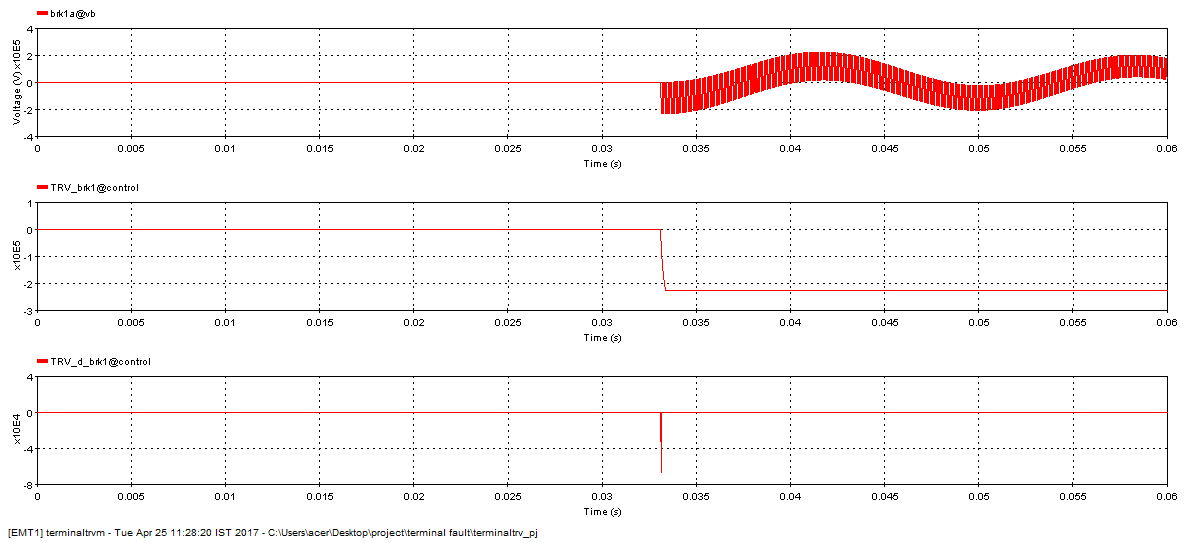
\includegraphics[width=\textwidth]{6trvawithstdcbp1416} 
   \caption{Phase A TRV, Standard TRV and Delay Line for Oscillatory TRV for Three Phase to Ground Terminal Fault for Transformer Switching}
   \label{Fig:4.1.6} 
\end{sidewaysfigure}

%***********************************************************************************************

\begin{sidewaysfigure}
   \centering 
   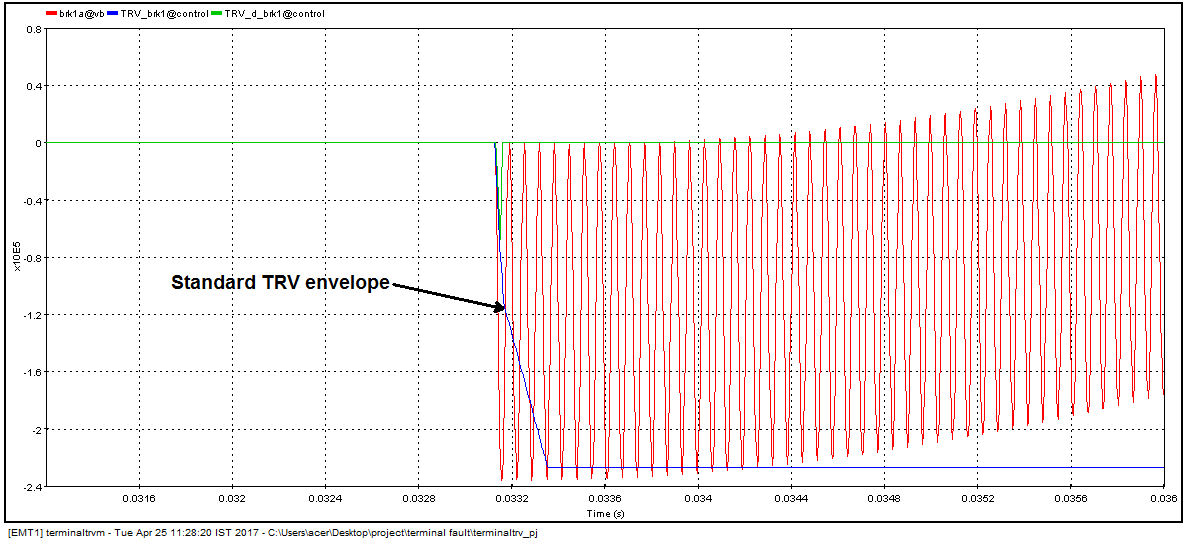
\includegraphics[width=\textwidth]{7trvawithstdenlargedcbp1417} 
   \caption{Enlarged View of Phase A TRV and Standard TRV Envelope for Three Phase to Ground Terminal Fault for Transformer Switching}
   \label{Fig:4.1.7} 
\end{sidewaysfigure}

%***********************************************************************************************

\begin{sidewaysfigure}
   \centering 
   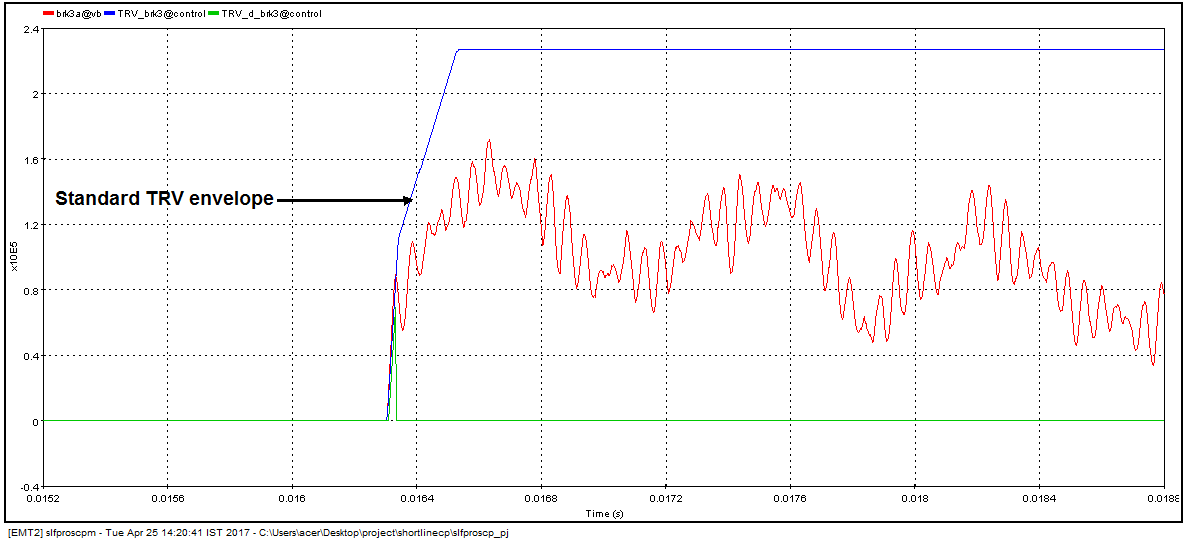
\includegraphics[width=\textwidth]{8slfcp418} 
   \caption{TRV for Short Line Single Phase to Ground Fault for Constant Parameter Model of Lines}
   \label{Fig:4.1.8} 
\end{sidewaysfigure}

%***********************************************************************************************

\begin{sidewaysfigure}
   \centering 
   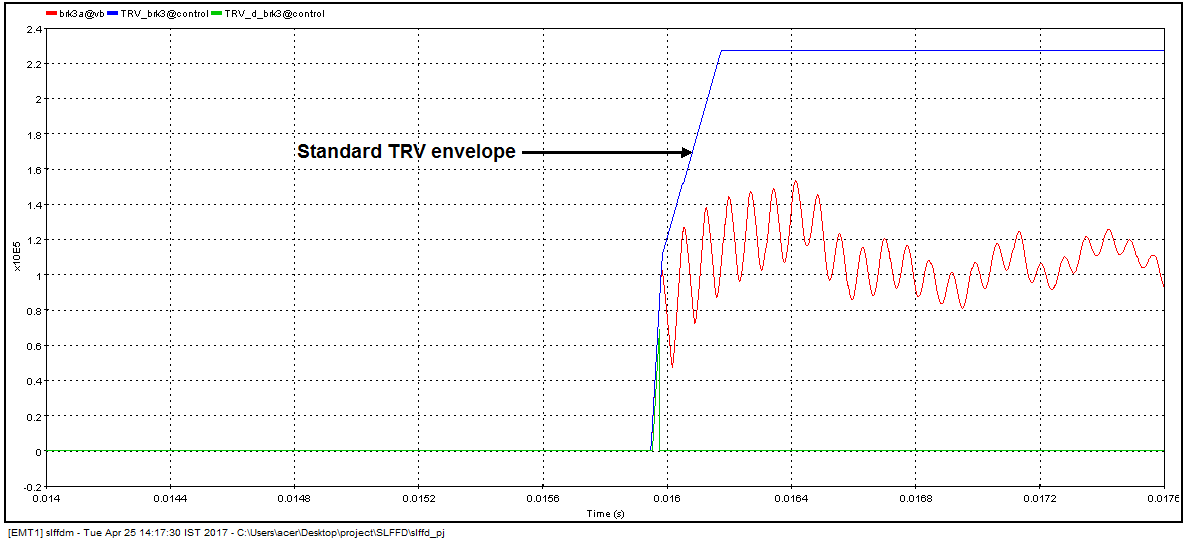
\includegraphics[width=\textwidth]{9slfd419} 
   \caption{TRV for Short Line Single Phase to Ground Fault for Frequency Dependent Model of Lines}
   \label{Fig:4.1.9} 
\end{sidewaysfigure}

%***********************************************************************************************

\begin{sidewaysfigure}
   \centering 
   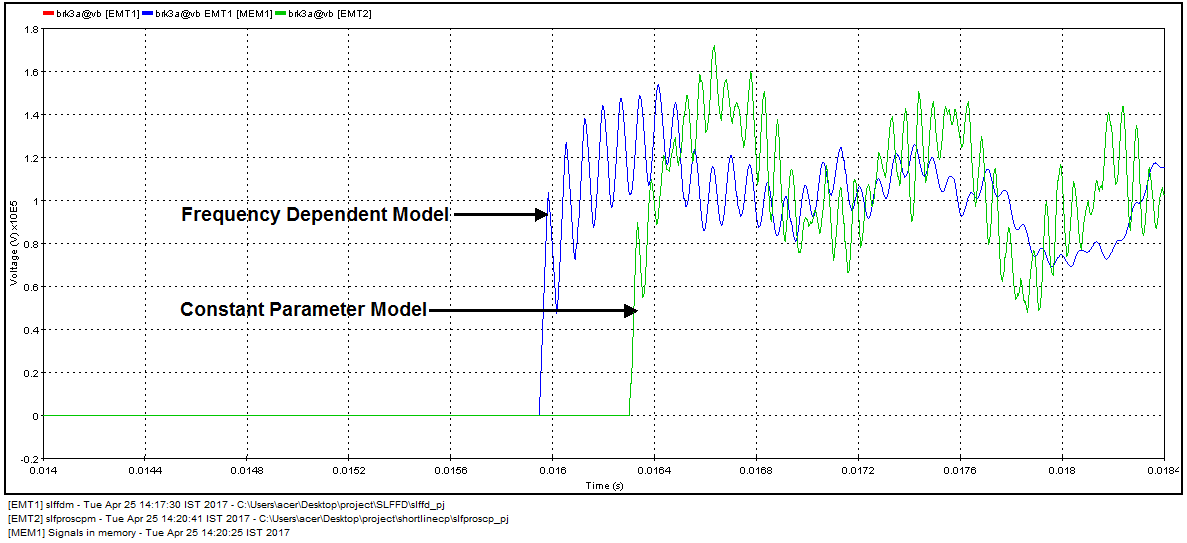
\includegraphics[width=\textwidth]{91slfdcpcombine4110} 
   \caption{Comparative Waveform of TRV for Constant Parameter Model and Frequency Dependent Model of Line for Short Line Single Phase to Ground }
   \label{Fig:4.1.10} 
\end{sidewaysfigure}
%*******************************************************************************************************
%********************************************************************************************************
\begin{sidewaysfigure}
   \centering 
   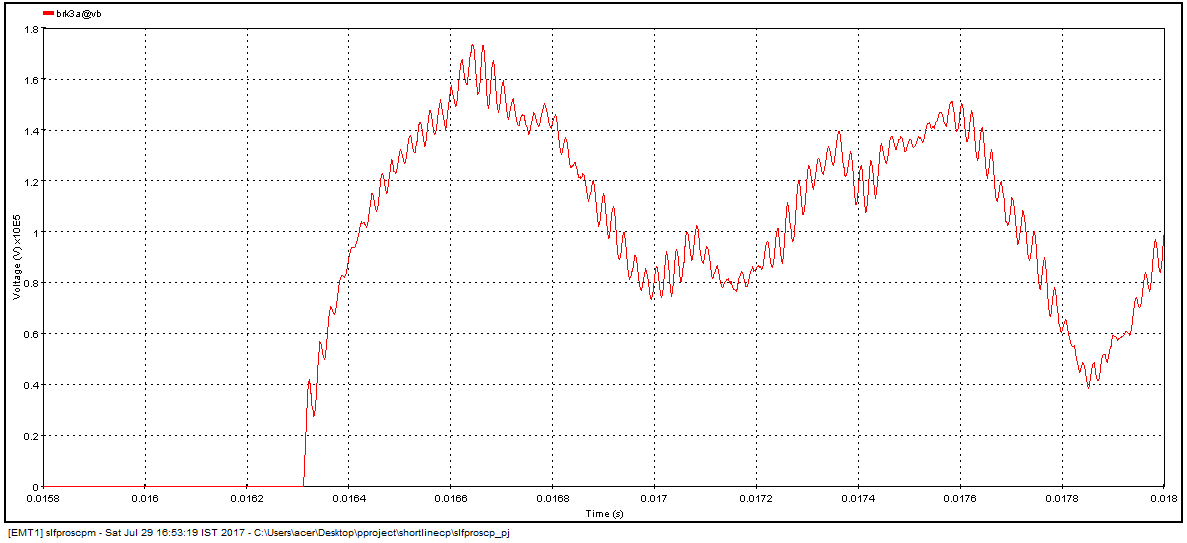
\includegraphics[width=\textwidth]{41112km} 
   \caption{TRV for Short Line Single Phase to Ground Fault at 1.2 km for Constant Parameter Model of Lines}
   \label{Fig:4.1.11} 
\end{sidewaysfigure}

\begin{sidewaysfigure}
   \centering 
   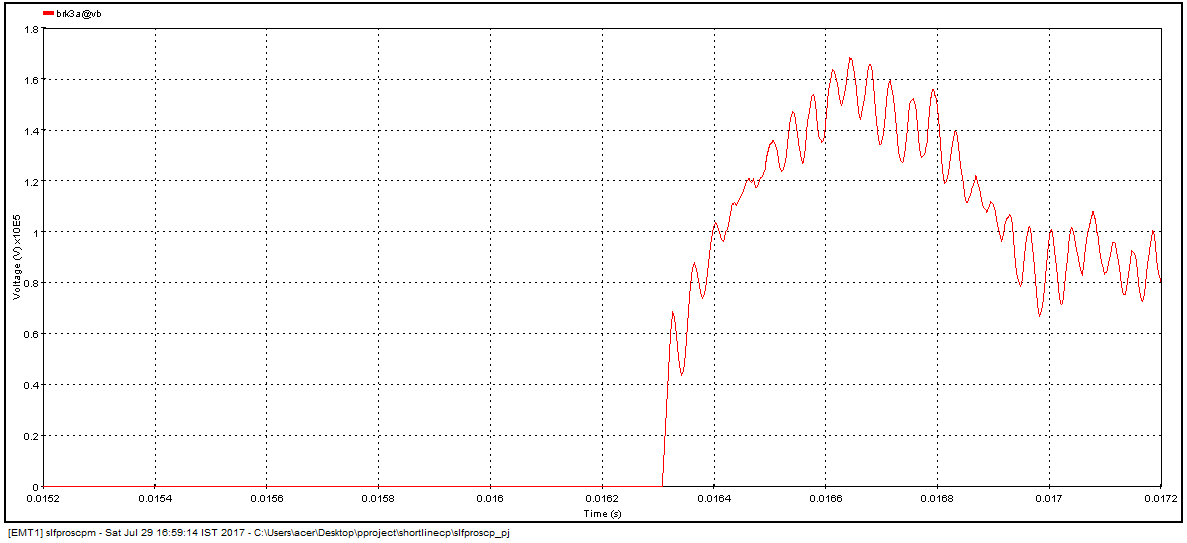
\includegraphics[width=\textwidth]{41222km} 
   \caption{TRV for Short Line Single Phase to Ground Fault at 2.2 km for Constant Parameter Model of Lines}
   \label{Fig:4.1.12} 
\end{sidewaysfigure}

\begin{sidewaysfigure}
   \centering 
   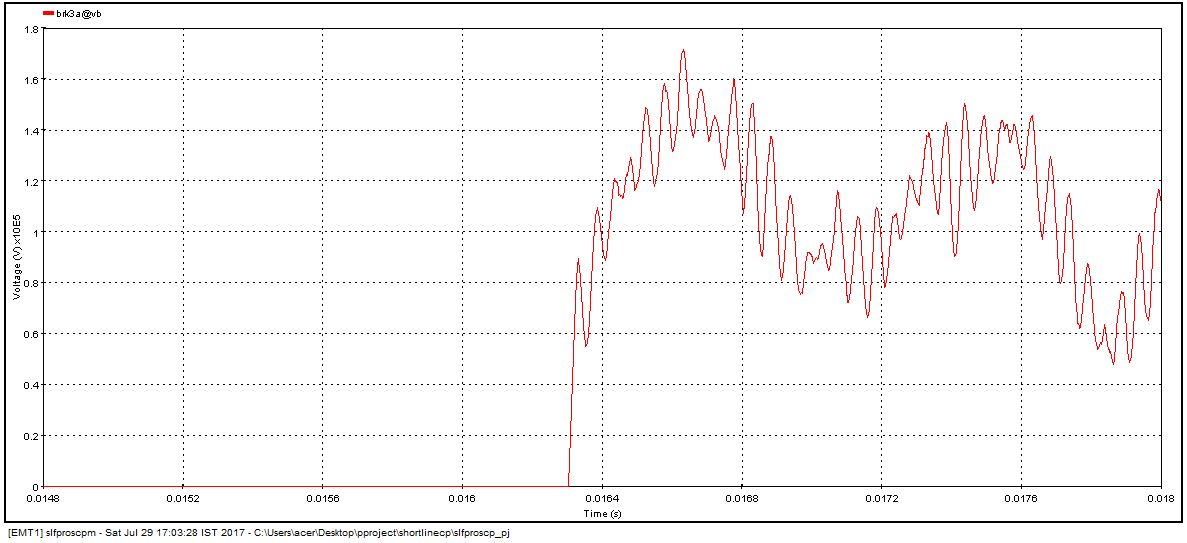
\includegraphics[width=\textwidth]{41332km} 
   \caption{TRV for Short Line Single Phase to Ground Fault at 3.2 km for Constant Parameter Model of Lines}
   \label{Fig:4.1.13} 
\end{sidewaysfigure}

\begin{sidewaysfigure}
   \centering 
   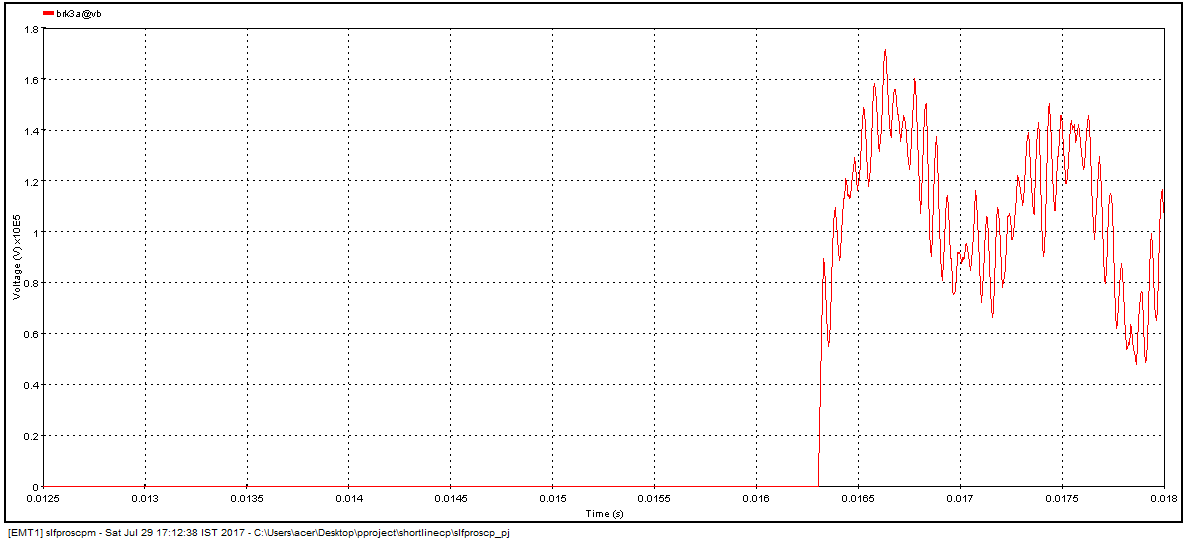
\includegraphics[width=\textwidth]{41452km} 
   \caption{TRV for Short Line Single Phase to Ground Fault at 5.2 km for Constant Parameter Model of Lines}
   \label{Fig:4.1.14} 
\end{sidewaysfigure}

\begin{sidewaysfigure}
   \centering 
   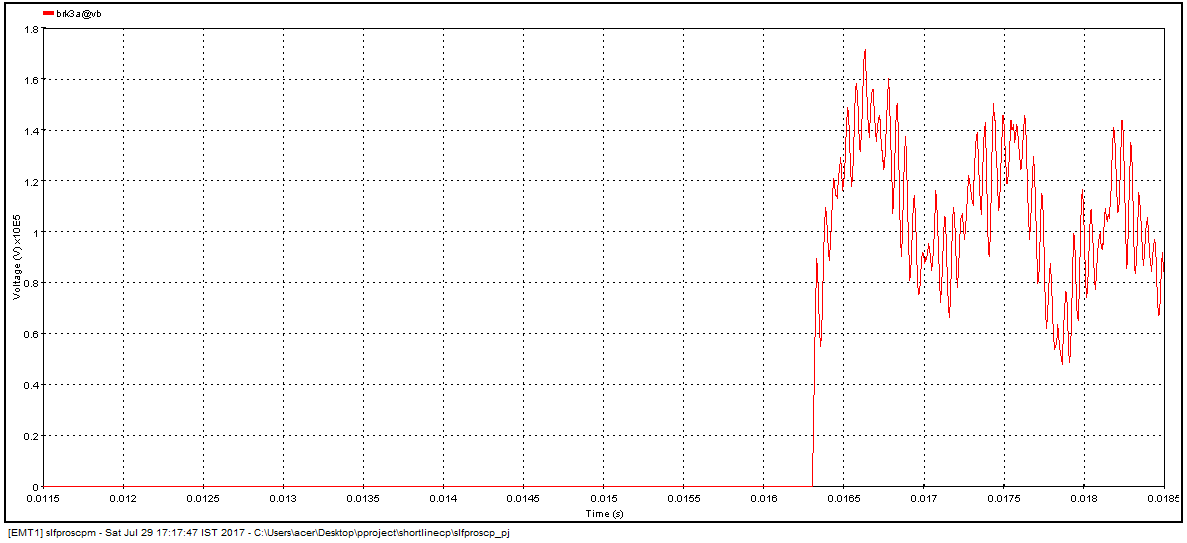
\includegraphics[width=\textwidth]{41562km} 
   \caption{TRV for Short Line Single Phase to Ground Fault at 6.2 km for Constant Parameter Model of Lines}
   \label{Fig:4.1.15} 
\end{sidewaysfigure}
%*************************************************************************************************
%***********************************************************************************************

\begin{sidewaysfigure}
   \centering 
   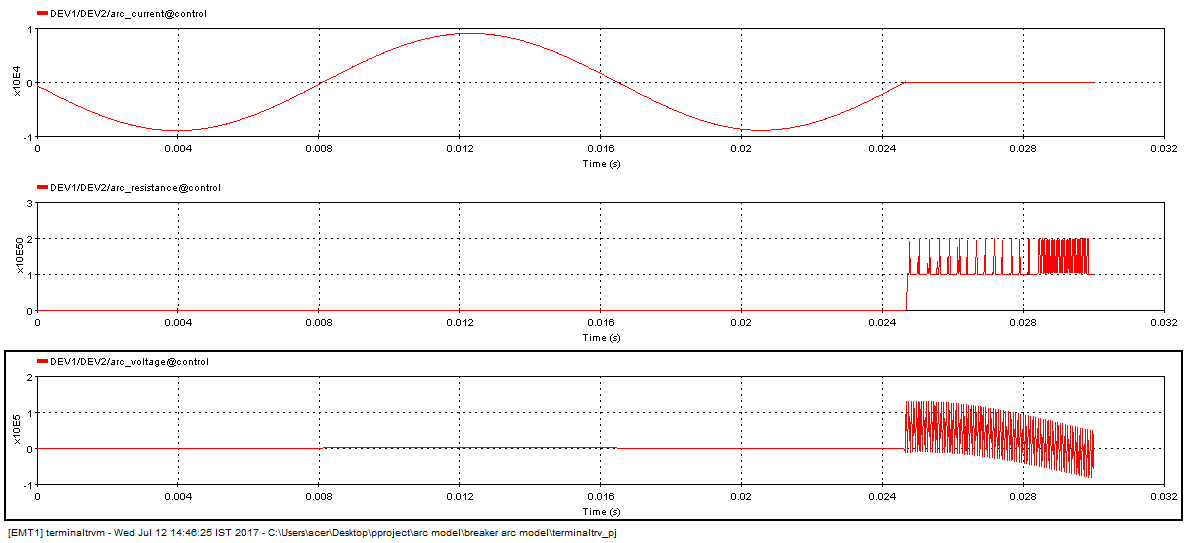
\includegraphics[width=\textwidth]{92transformerp44111} 
   \caption{Arc Interruption Waveforms for Three Phase to Ground Terminal Fault for Transformer Switching}
   \label{Fig:4.1.16} 
\end{sidewaysfigure}

%***********************************************************************************************

\begin{sidewaysfigure}
   \centering 
   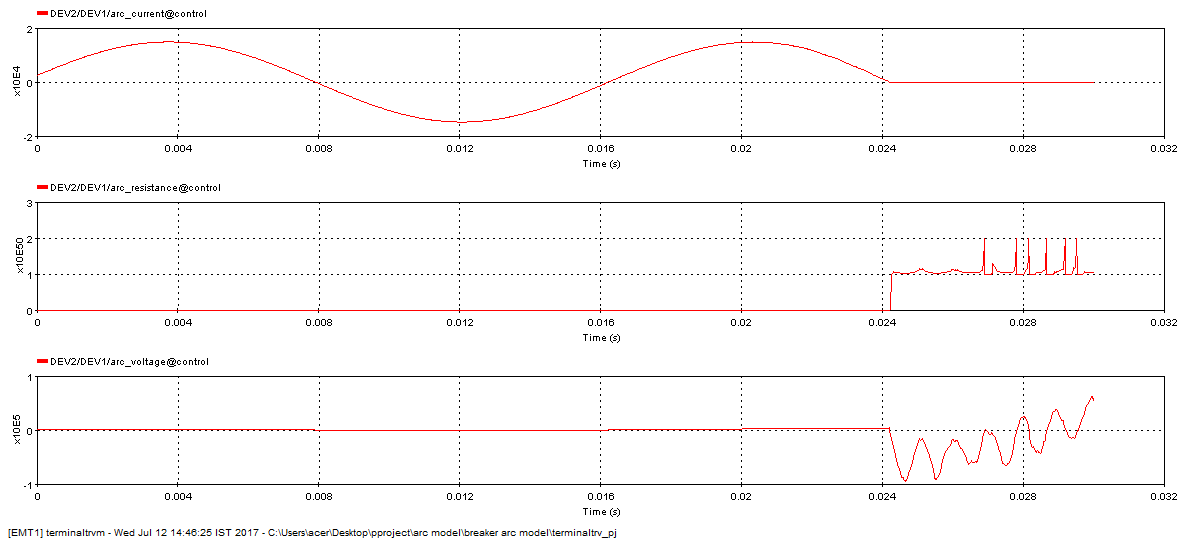
\includegraphics[width=\textwidth]{93transformerp54112} 
   \caption{Arc Interruption Waveforms for Three Phase to Ground Terminal Fault for Multiple Line Switching}
   \label{Fig:4.1.17} 
\end{sidewaysfigure}

%***********************************************************************************************
\clearpage

\section{Analytical Analysis}
Based on the developed system discussed in chapter 3, comprehensive analytical analysis is done for the following models considering and solving the mathematical equations \ref{eq:3.1} to \ref{eq:3.11}.

\begin{enumerate}
\item The network under study is modeled for three phase to ground fault at the terminal of substation for switching multiple lines connected to the substation. Equations \ref{eq:3.1} to  \ref{eq:3.5} modeling the system for this condition give the short circuit current of 17.1 kA under steady state conditions which is closed to the 17.2 kA obtained through simulation. The RRRV obtained analytically through equation  \ref{eq:3.6} is 0.91 kV/$\mu s$ which is close to 1.2 kV/$\mu s$ obtained through simulation. 

\item The network under study is modeled for three phase to ground fault at the terminal of substation for transformer switching. Equations \ref{eq:3.1} to \ref{eq:3.3} and \ref{eq:3.7} used to find RRRV gave the value of 6.75 kV/$\mu s$ which is in close approximation to 7.65 kV/$\mu s$ obtained through simulation.

\item The network is modeled for single phase to ground short line fault using constant parameter mode as well as frequency dependent mode of transmission line. Equations \ref{eq:3.8} to \ref{eq:3.11} give the RRRV 2.87 kV/$\mu s$ which is in good agreement with the simulated value of 2.35 kV/$\mu s$ for a fault at 4.2 km. The RRRV is plotted for different fault distance in the figure \ref{fig:Variation of RRRV with Fault Distance for Single Phase to Ground Short Line Fault}. It is observed that the RRRV increases with reduction in fault distance.

\item The network under study is modeled for three phase to ground fault at the terminal of substation for multiple lines switching as well as transformer switching. Black Box model using Cassie-Mayer equations is used for arc interruption studies. Successful interruption of arc is observed in both cases.
\end{enumerate}

\begin{figure}[!htbp]
    \centering
    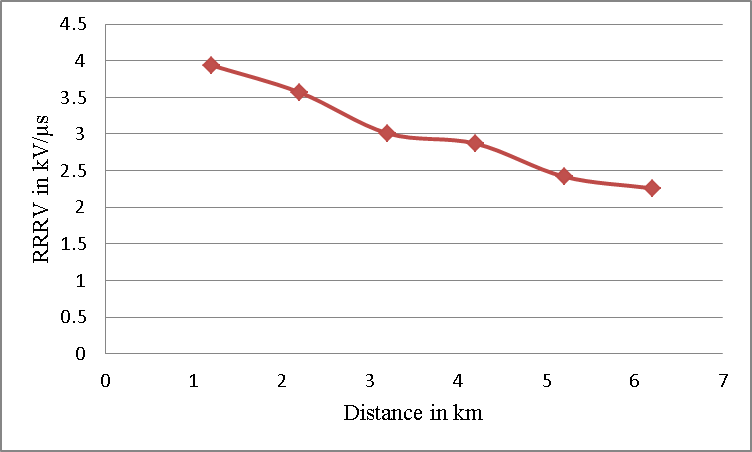
\includegraphics[width=\textwidth]{VariationofRRRVwithFaultDistance}
    \caption{Variation of RRRV with Fault Distance for Single Phase to Ground Short Line Fault}
    \label{fig:Variation of RRRV with Fault Distance for Single Phase to Ground Short Line Fault}
\end{figure}

\section[Comparison between Computational and Analytical Analysis]{Comparison between Computational and\\Analytical Analysis}
1. Short circuit current during Three Phase to Ground fault through simulation is found to be 17.2 kA which is almost same (17.1 kA) as obtained analytically.

2. Table \ref{table:Comparison of Standard TRV and Simulated TRV} gives the parameters of standard TRV and TRV obtained through simulation

\centering
\begin{table}[!htbp]
\begin{center}
\begin{threeparttable}
\caption{Comparison of Standard TRV and Simulated TRV}
\label{table:Comparison of Standard TRV and Simulated TRV}
\begin{tabular}{| l | c | c | c | c | c | c | c | c |}
\hline
{~}	&\textbf{$u_1$}&\textbf{$t_1$}&\textbf{$u_c$}&\textbf{$t_2$}&\textbf{$t_d$}&\textbf{$u^\prime$}&\textbf{$t^\prime$}&\textbf{$u_1/t_1$}\\

{~}&\textbf{$kV$}&\textbf{$\mu s$}&\textbf{$kV$}&\textbf{$\mu s$}&\textbf{$\mu s$}&\textbf{$kV$}&\textbf{$\mu s$}&\textbf{$kV/\mu s$}\\ \hline
Standard&115&38&231&228&2-12&58&21-31&3\\ \hline
Simulated&114.8&39&230&227.4&3.2&58.2&26&2.9\\ \hline
\end{tabular}
\end{threeparttable}
\end{center}
\end{table}

\justify
3.	Table \ref{table:Simulation Results for TRV under Different Fault Conditions} shows the max. Value of TRV and RRRV under different fault conditions.

\begin{table}[!htbp]
\renewcommand{\arraystretch}{1}
\caption{Simulation Results for TRV under Different Fault Conditions}
\label{table:Simulation Results for TRV under Different Fault Conditions}
\centering
\small
\begin{tabular}{| >{\arraybackslash}m{0.2in} | >{\arraybackslash}m{1.7in} | >{\arraybackslash}m{0.7in} | >{\arraybackslash}m{0.6in} | >{\arraybackslash}m{0.65in} | >{\arraybackslash}m{1.1in} |} \hline

\multirow{2}{*}{Sr.} & \multirow{2}{*}{Type of fault} & \multirow{2}{*}{Max.Value} &\multicolumn{2}{|c|}{RRRV (kV/$\mu s$)} & \multirow{2}{*}{Nature of TRV} \\ \cline{4-5}
{No.}&{}&{of~TRV (kV)}& Simulated & Analytical &{} \\ \hline
\multirow{3}{*}{1} & Three Phase to Ground fault at the terminal of substation &{}&{}&{}&{}\\
 & (a) Multiple lines connected to bus & 182.215 & 1.2 & 0.91 & (a)Exponential as
per standard \\
&(b)Transformer switching & 235.855 & 7.65 & 6.75 & (b) Oscillatory as per standard \\ \hline

\multirow{3}{*}{2} & Short line fault &{}&{}&{}&{}\\
&(a)Constant parameter model &171.65&2.89&2.87&Saw tooth shaped as per\\

&(b)Frequency dependent model & 153.53 &2.5 &{} & standard \\ \hline
\end{tabular}
\end{table}

\justify
\section{Validation of Algorithm}
The proposed algorithm is applied to the case study \cite{salamanca1993preventive}. One new fixed contact ($F_1$) and four moving contacts, relatively new contact ($M_1$), slightly worn contact ($M_2$) a worn contact ($M_3$) and seriously damaged worn contact ($M_4$) as shown in figure \ref{fig:Fix and Moving Contacts with Different Worn Conditions} were considered. Figure \ref{fig:DCRM Signature in the Trip Portion for Different Contact Configuration [67]} shows the DCRM of the tripping portion. The value of $A_a$, area below the arcing contact region is shown in table \ref{table:Area below the DCRM Curve for Different Contact Configuration [67]}.

Value of $\Delta T_a$, $\Delta T_m$, $\Delta A_m$ and $\Delta R_{aimax}$ is not measured. But as seen from the graph in figure \ref{fig:DCRM Signature in the Trip Portion for Different Contact Configuration [67]}, $\Delta T_a \cong 0$, $\Delta T_m \cong 0$, $\Delta R_{aimax} > 0$ and $\Delta A_m \cong 0$ and $\Delta A_a > 0$. when this data is fed to the proposed algorithm, it detects problem no. 3 that corresponds to wearing of moving contact which is same as proposed in the algorithm.

\begin{figure}
    \centering
    \begin{subfigure}[b]{0.3\textwidth}
        \centering
        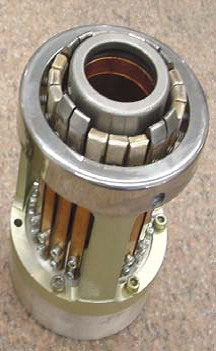
\includegraphics[width=\textwidth, height= 8cm]{k1RelativelyNewFixed}
        \caption{Relatively New Fixed Contact (F1)}
        \label{fig:Relatively New Fixed Contact}
    \end{subfigure}
    \begin{subfigure}[b]{0.3\textwidth}
        \centering
        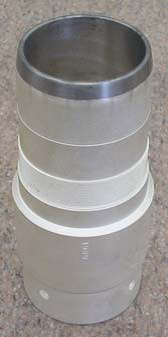
\includegraphics[width=\textwidth, height= 8cm]{k2NewMovingContact}
        \caption{New Moving Contact (M1)}
        \label{fig:New Moving Contact}
    \end{subfigure}
    \begin{subfigure}[b]{0.3\textwidth}
        \centering
        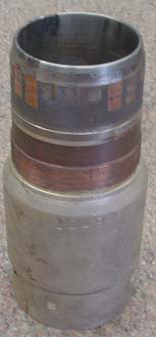
\includegraphics[width=\textwidth, height= 8cm]{k3SlightlyWornMoving}
        \caption{Slightly Worn Moving Contact (M2)}
        \label{fig:Slightly Worn Moving Contact}
    \end{subfigure}
    \\
    \begin{subfigure}[b]{0.3\textwidth}
        \centering
        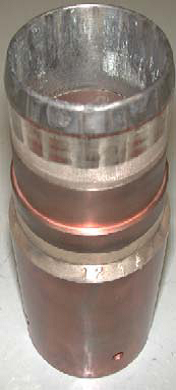
\includegraphics[width=\textwidth, height= 8cm]{k4WornMovingContact}
        \caption{Worn Moving Contact (M3)}
        \label{fig:Worn Moving Contact}
    \end{subfigure}
    \begin{subfigure}[b]{0.3\textwidth}
        \centering
        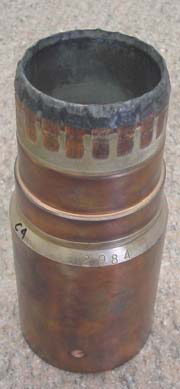
\includegraphics[width=\textwidth, height= 8cm]{k5SeriouslyWornMovingContact}
        \caption{Seriously Worn Moving Contact (M4)}
        \label{fig:Seriously Worn Moving Contact}
    \end{subfigure}
    \caption[Fix and Moving Contacts with Different Worn Conditions]{Fix and Moving Contacts with Different Worn Conditions \cite{salamanca1993preventive}}
    \label{fig:Fix and Moving Contacts with Different Worn Conditions}
\end{figure}

\begin{figure}[!htbp]
\centering
\begin{minipage}{\textwidth}
\centering
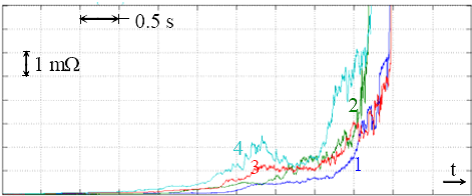
\includegraphics[width=\textwidth]{DCRMSignatureintheTripPortion}
\begin{center}
\footnotesize \textcolor{Blue}{1: Contact set F1-M1}; \textcolor{OliveGreen}{2: Contact set F1-M2}; \textcolor{Red}{3: Contact set F1-M3}; \textcolor{Cerulean}{4: Contact set F1-M4}
\end{center}
\end{minipage}
\caption[DCRM Signature in Trip Portion for Different Contact Configuration]{DCRM Signature in the Trip Portion for Different Contact Configuration \cite{salamanca1993preventive}}
\label{fig:DCRM Signature in the Trip Portion for Different Contact Configuration [67]}
\end{figure}

\begin{table}[!htbp]
\renewcommand{\arraystretch}{1.3}
\begin{center}
\caption[Area below the DCRM Curve for Different Contact Configuration]{Area below the DCRM Curve for Different Contact Configuration \cite{salamanca1993preventive}}
\label{table:Area below the DCRM Curve for Different Contact Configuration [67]}
\begin{tabular}{| >{\centering\arraybackslash}m{2in} | >{\centering\arraybackslash}m{2in} | }
\hline
Contact set	&	$A_a ( m\Omega.s)$	\\ \hline
$F_1 - M_1$		&	2.7			\\ \hline
$F_1 - M_2$		&	2.8			\\ \hline
$F_1 - M_3$		&	3.9			\\ \hline
$F_1 - M_4$		&	5.4			\\ \hline
\end{tabular}
\end{center}
\end{table}

\clearpage
Figure \ref{fig:Signatures of R-pole from Commissioning}a - d shows the DCRM signatures of R-pole of a 400 kV SF\textsubscript{6} circuit breaker from commissioning stage. Large variations of resistance in the no action zone are seen in the DCRM signature on 15/12/2014. Table \ref{table:CB Parameters for the Healthy and Faulty Condition from DCRM Signature} shows the CB parameters for the healthy and faulty condition from DCRM signature. When the parameters are fed, the algorithm detected problem of main contact erosion. Figure \ref{fig:Output of the Program} shows the output of the program. It is confirmed by the static contact resistance test which gave a very high value of static contact resistance 170 $\mu \Omega$.

\begin{table}[!htbp]
\renewcommand{\arraystretch}{1.3}
\begin{center}
\caption{CB Parameters for the Healthy and Faulty Condition from DCRM Signature}
\label{table:CB Parameters for the Healthy and Faulty Condition from DCRM Signature}
\begin{tabular}{| >{\arraybackslash}m{1in} | >{\centering\arraybackslash}m{0.75in} |>{\centering\arraybackslash}m{0.75in} |>{\centering\arraybackslash}m{0.75in} |>{\centering\arraybackslash}m{0.75in} |>{\centering\arraybackslash}m{0.75in} | }
\hline
Description		& $T_m$ & $T_a$ & $R_{iam}$ 	& $A_m$ 			& $A_a$ \\
{~} 			&(ms)	& (ms)	&($\mu \Omega$)	& ($\mu \Omega \times$ms)	& ($\mu \Omega \times$ms)\\ \hline
Current Value	& 315.6	& 318.9	& 860			& 30430				& 1665			   \\ \hline
Base Value		& 316.8	& 318.9	& 860			& 6120				& 886.2				\\ \hline
Difference $\Delta$&-1.2& 0		& 0				& 24310				& 778.8				\\ \hline
\end{tabular}
\end{center}
\end{table}

Figure \ref{fig:Signatures of Y-pole from Commissioning}a - d shows the DCRM signatures of Y-pole of the same circuit breaker from commissioning stage. Spike is seen in close zone portion of the signature. When algorithm is applied step by step, the problem of contact wipe is detected. The contact wipe was found to be 16 mm. When contact wipe is adjusted to specified limit, normal DCRM signature is obtained as shown in figure \ref{fig:Signature on 15/12/2014 After Wipe Adjustment}.

\begin{figure}
    \centering
    \begin{subfigure}[b]{\textwidth}
        \centering
        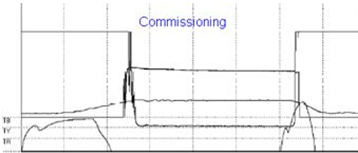
\includegraphics[width=8cm, height=5cm]{l1SignatureatCommissioning}
        \caption{Signature at Commissioning}
        \label{fig:Signature at Commissioning}
    \end{subfigure}
    \\
    \begin{subfigure}[b]{\textwidth}
        \centering
        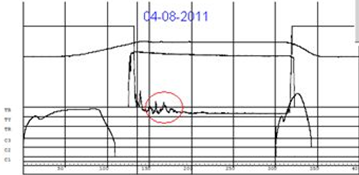
\includegraphics[width=8cm, height=5cm]{l2Signatureon482011}
        \caption{Signature on 4/8/2011}
        \label{fig:Signature on 4/8/2011}
    \end{subfigure}
    \\
    \begin{subfigure}[b]{\textwidth}
        \centering
        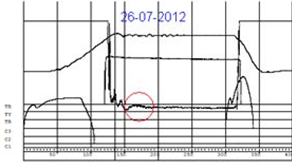
\includegraphics[width=8cm, height=5cm]{l3Signatureon2672012}
        \caption{Signature on 26/7/2012}
        \label{fig:Signature on 26/7/2012}
    \end{subfigure}
    \\
    \begin{subfigure}[b]{\textwidth}
        \centering
        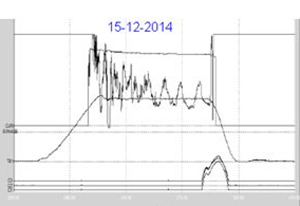
\includegraphics[width=8cm, height=5cm]{l4Signatureon15122014}
        \caption{Signature on 15/12/2014}
        \label{fig:Signature on 15/12/2014}
    \end{subfigure}
    
    \caption{Signatures of R-pole from Commissioning}
    \label{fig:Signatures of R-pole from Commissioning}
\end{figure}

\begin{figure}[!htbp]
    \centering
    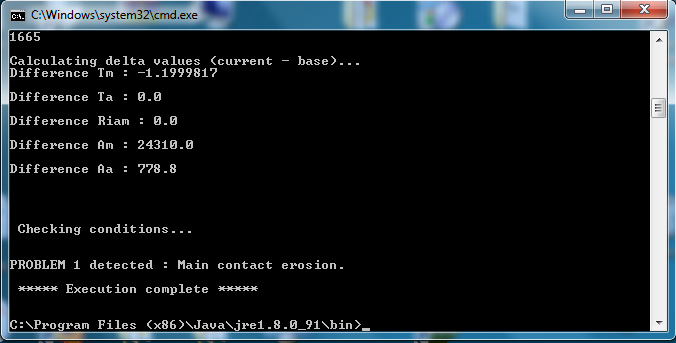
\includegraphics[width=\textwidth]{OutputoftheProgram}
    \caption{Output of the Program}
    \label{fig:Output of the Program}
\end{figure}

\begin{figure}
    \centering
    \begin{subfigure}[b]{\textwidth}
        \centering
        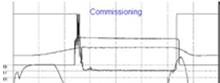
\includegraphics[width=8cm, height=5cm]{m1SignatureatCommissioning}
        \caption{Signature at Commissioning}
        \label{fig:Signature at Commissioning n}
    \end{subfigure}
    \\
    \begin{subfigure}[b]{\textwidth}
        \centering
        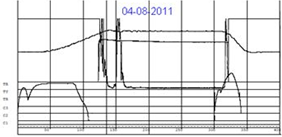
\includegraphics[width=8cm, height=5cm]{m2Signatureon482011}
        \caption{Signature on 4/8/2011}
        \label{fig:Signature on 4/8/2011n}
    \end{subfigure}
    \\
    \begin{subfigure}[b]{\textwidth}
        \centering
        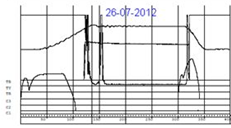
\includegraphics[width=8cm, height=5cm]{m3Signatureon2672012}
        \caption{Signature on 26/7/2012}
        \label{fig:Signature on 26/7/2012n}
    \end{subfigure}
    \\
    \begin{subfigure}[b]{\textwidth}
        \centering
        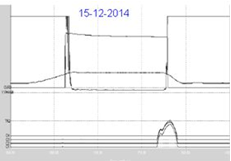
\includegraphics[width=8cm, height=5cm]{m4Signatureon15122014}
        \caption{Signature on 15/12/2014 After Wipe Adjustment}
        \label{fig:Signature on 15/12/2014 After Wipe Adjustment}
    \end{subfigure}
    
    \caption{Signatures of Y-pole from Commissioning}
    \label{fig:Signatures of Y-pole from Commissioning}
\end{figure}

\clearpage
\section{Justification for Difference}
The difference in the results obtained is because of the round off of the parameters in decimals. The nature of TRV obtained for different fault conditions is in good agreement with the standard waveforms available in the literature. Improper placement of the travel transducer or linkage ratio results in error in the DCRM signature. ~Induction effect in the substation ~switching yard ~also affects ~the measurement. DCRM must be taken with the same sampling frequency, resistance range and plot length so as to compare for variation. Change in any of the setting details for data acquisition will lead to variation in the signature which makes it difficult for comparison.